\documentclass{standalone}
\usepackage{tikz}
\usetikzlibrary{mindmap, backgrounds, trees}

\begin{document}
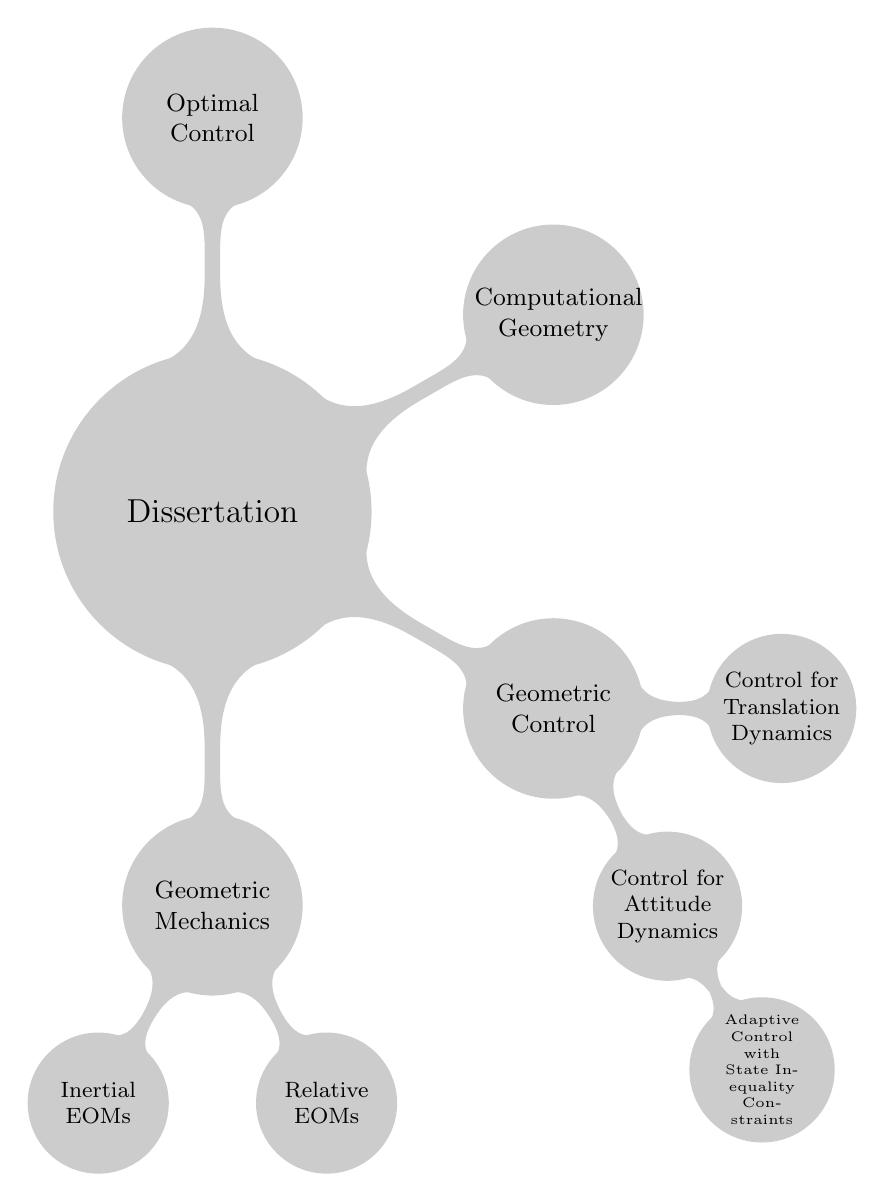
\begin{tikzpicture}[
    mindmap, every node/.style=concept,
    grow cyclic,
    concept color=black!20,
    ]
    \node [root concept] {Dissertation} % root
            child { node {Geometric Mechanics}
                child { node { Inertial EOMs} }
                child { node {Relative EOMs} }
            }
            child { node {Geometric Control}
                child { node { Control for Attitude Dynamics} 
                    child { node { Adaptive Control with State Inequality Constraints } } 
                }
                child { node { Control for Translation Dynamics} }
             }
            child { node {Computational Geometry} }
            child { node {Optimal Control} }; 
    \end{tikzpicture}
\end{document}
